% ============================================================
%  SECTION 3 — PROBLEM FORMULATION
% ============================================================
This section develops the formal problem structure for portfolio-level budget
allocation in contracted project portfolios. The formulation proceeds across
three levels. \textbf{Level~1} (Section~\ref{subsec:level1}) treats all
contractor performance parameters as known and establishes the deterministic
MILP whose optimum constitutes a theoretical upper bound: no implementable
policy operating under uncertainty can exceed it.
\textbf{Level~2} (Section~\ref{subsec:level2}) reintroduces stochastic
efficiency and characterizes the resulting multi-stage stochastic program,
establishing that its scenario tree grows exponentially in the number of
projects and periods. \textbf{Level~3} (Section~\ref{subsec:level3})
reformulates the intractable stochastic program as a Constrained Markov
Decision Process (CMDP), providing an explicit mapping from LP elements to MDP
primitives and yielding a Gymnasium-compatible environment on which the PPO
agent of Section~\ref{sec:experiments} is trained. The three levels are a
coherent arc --- Level~1 defines the ceiling, Level~2 explains why it is
unreachable, Level~3 provides the tractable path --- all sharing the primitives
defined next.

% ------------------------------------------------------------
\subsection{Scope, Assumptions, and Problem Primitives}
\label{subsec:primitives}
% ------------------------------------------------------------

\paragraph{Scope.}
The problem is operational, not strategic: the portfolio of contracted projects
is fixed, commitments are signed, and the decision-maker exercises a single
lever --- the budget $x_{i,t}$ directed to each active project $i$ at each
discrete period $t$. All outcomes of interest (milestone achievement, cash
balance, schedule adherence, termination) flow through this allocation decision.
Portfolio selection is treated as exogenous \cite{Archer1999}.

\paragraph{Structural assumptions.}
Four choices underlie the entire formulation.
(i)~\emph{Independent bilateral contracts}: projects interact only through the
shared budget constraint; no resource or workforce sharing occurs, consistent
with standard EPC contracting practice.
(ii)~\emph{Budget as the sole control}: the contractor's internal resource
decisions are absorbed into the efficiency parameter $\eta_{i,t}$; the
portfolio manager observes only how much physical progress a budget allocation
yields, not how it is achieved.
(iii)~\emph{Discrete monthly periods}: $\mathcal{T} = \{1,\ldots,H\}$
reflects the monthly governance cycle of portfolio management (progress
reporting, payment certification, performance review).
(iv)~\emph{FIDIC contract mechanics}: the milestone payment structure, advance
payment and recovery, retention, and termination settlement are parameterized
consistently with FIDIC Red, Yellow, and Silver Book forms
\cite{FIDIC2017}; all contract-specific quantities are calibrated
parameters, not fixed constants.

% - - - - - - - - - - - - - - - - - - - - - - - - - - - - - -
\subsubsection{Sets, Indices, and the Decision Variable}
\label{subsubsec:sets}
% - - - - - - - - - - - - - - - - - - - - - - - - - - - - - -

\begin{description}[leftmargin=2.2cm, labelwidth=2.0cm]
  \item[$\mathcal{P}$]
    Projects $\{1,\ldots,n\}$, indexed by $i$; all committed at horizon start.
  \item[$\mathcal{T}$]
    Planning periods $\{1,\ldots,H\}$, indexed by $t$ (calendar months).
  \item[$\mathcal{M}_i$]
    Ordered milestones $\{1,\ldots,M_i\}$ for project $i$, indexed by $j$,
    with thresholds $\theta_{i,1} < \cdots < \theta_{i,M_i} = 1$.
  \item[$\mathcal{A}_i^{\mathrm{plan}}$]
    Planned execution window $\{s_i,\ldots,f_i\}$; anchors S-curve computations.
  \item[$\mathcal{P}_t^{\mathrm{active}}$]
    Projects active at period $t$; fixed parameter at Level~1, endogenous at
    Levels~2--3.
  \item[$\mathcal{M}_i^{\mathrm{cert}}(t)$]
    Milestones of project $i$ certified by period $t$:
    $\{j : \theta_{i,j} \leq P_{i,t}^{\mathrm{actual}}\}$.
  \item[$x_{i,t} \geq 0$]
    \textbf{Decision variable}: budget allocated to project $i$ at period $t$.
    The period-$t$ action is $\mathbf{x}_t = (x_{i,t})_{i \in
    \mathcal{P}_t^{\mathrm{active}}}$.
  \item[$B_t \geq 0$]
    Portfolio cash balance at the start of period $t$; $B_1$ is given.
\end{description}

% - - - - - - - - - - - - - - - - - - - - - - - - - - - - - -
\subsubsection{Project Parameters}
\label{subsubsec:project_params}
% - - - - - - - - - - - - - - - - - - - - - - - - - - - - - -

Tables~\ref{tab:params-schedule-contract} and~\ref{tab:params-cost-penalty}
list all project parameters, fixed at commitment. The planned cumulative
expenditure fraction follows a normalized S-curve
\cite{Kenley2009,barraza2004probabilistic} parameterized by
$(a_i,b_i)$:
\[
  P_{i,t}^{\mathrm{plan}} = F_i(\tau_{i,t}^c) = I_{\tau_{i,t}^c}(a_i, b_i),
  \qquad
  \tau_{i,t} = \frac{t - s_i + 1}{D_i^{\mathrm{plan}}},
  \quad
  \tau_{i,t}^c = \min\{1,\max\{0,\tau_{i,t}\}\},
\]
where $I_\tau(\cdot,\cdot)$ is the regularized incomplete Beta function.
The planned period expenditure increment is
$\Delta\bar{E}_{i,t} = \mathrm{BAC}_i\,[F_i(\tau_{i,t}^c) - F_i(\tau_{i,t-1}^c)]$.
This profile is a fixed parameter derived at commitment from
$(a_i, b_i, s_i, f_i, \mathrm{BAC}_i)$; it is never a decision variable.

\begin{table}[H]
  \centering\small
  \renewcommand{\arraystretch}{1.3}\setlength{\tabcolsep}{8pt}
  \begin{tabular}{>{\bfseries}p{3.4cm} p{2.0cm} p{1.3cm} p{7.0cm}}
    \toprule
    \normalfont\textbf{Parameter} & \textbf{Symbol} & \textbf{Domain} & \textbf{Definition} \\
    \midrule
    \rowcolor{RowAlt}
    Planned start \& finish \newline\tagschedule
      & $s_i,\;f_i$ & $\mathbb{Z}^+$
      & Anchor of execution window $\mathcal{A}_i^{\mathrm{plan}}$ and S-curve. \\
    Planned duration \newline\tagschedule
      & $D_i^{\mathrm{plan}}$ & $\mathbb{Z}^+$
      & $f_i - s_i + 1$; normalizes progress against plan. \\
    \rowcolor{RowAlt}
    S-curve shape \newline\tagschedule
      & $a_i,\;b_i$ & $\mathbb{R}^+$
      & Beta CDF parameters governing the planned expenditure profile. \\
    Milestone threshold \newline\tagschedule
      & $\theta_{i,j}$ & $(0,1]$
      & Cumulative progress fraction required to certify milestone $j$. \\
    \rowcolor{RowAlt}
    Delay buffer \newline\tagschedule
      & $\mathrm{buffer}_i$ & $\mathbb{Z}^+_0$
      & Periods beyond $f_i$ before forced termination is assessed. \\
    \midrule
    Contract price \newline\tagcontract
      & $CP_i$ & $\mathbb{R}^+$
      & Total client payment; $CP_i = \mathrm{BAC}_i(1+\pi_i)$. \\
    \rowcolor{RowAlt}
    Profit margin \newline\tagcontract
      & $\pi_i$ & $\mathbb{R}^+_0$
      & Contractual markup on $\mathrm{BAC}_i$. \\
    Advance payment ratio \newline\tagcontract
      & $\alpha_i$ & $[0,1]$
      & $A_i = \alpha_i \cdot CP_i$ received at $t = s_i$; recovered through
        percentage deductions from subsequent interim payment certificates at
        rate $\delta_i^{\mathrm{rec}}$ once cumulative certified payments
        exceed threshold $\psi_i$ \citep{FIDIC2017}. \\
    \rowcolor{RowAlt}
    Recovery deduction rate \newline\tagcontract
      & $\delta_i^{\mathrm{rec}}$ & $(0,1]$
      & Fraction of each interim payment certificate deducted toward advance
        recovery once the commencement threshold $\psi_i$ is exceeded. \\
    Recovery commencement threshold \newline\tagcontract
      & $\psi_i$ & $[0,1]$
      & Cumulative certified interim payments as a fraction of $CP_i$ at which
        advance recovery deductions begin; default 0.10 under FIDIC
        Sub-Clause~14.2 \citep{FIDIC2017}. \\
    \rowcolor{RowAlt}
    Retention ratio \newline\tagcontract
      & $\rho_i$ & $[0,1]$
      & Fraction withheld per milestone; released as $R_i^{\mathrm{ret}} = \rho_i \cdot CP_i$ at completion. \\
    Milestone weight \newline\tagcontract
      & $\phi_{i,j}$ & $\mathbb{R}^+$
      & Fraction of $CP_i$ at milestone $j$; $\sum_j \phi_{i,j} = 1$. \\
    \bottomrule
  \end{tabular}
  \caption{Schedule and contract parameters for project $i \in \mathcal{P}$ (fixed at commitment).}
  \label{tab:params-schedule-contract}
\end{table}

\begin{table}[H]
  \centering\small
  \renewcommand{\arraystretch}{1.3}\setlength{\tabcolsep}{8pt}
  \begin{tabular}{>{\bfseries}p{3.4cm} p{2.0cm} p{1.3cm} p{7.0cm}}
    \toprule
    \normalfont\textbf{Parameter} & \textbf{Symbol} & \textbf{Domain} & \textbf{Definition} \\
    \midrule
    \rowcolor{RowAlt}
    Budget at completion \newline\tagcost
      & $\mathrm{BAC}_i$ & $\mathbb{R}^+$
      & Total planned contractor expenditure; EVM cost basis. \\
    Discount factor \newline\tagcost
      & $\gamma$ & $(0,1]$
      & Per-period discount applied to future cash flows; shared across $\mathcal{P}$. \\
    \rowcolor{RowAlt}
    Initial cash balance \newline\tagcost
      & $B_1$ & $\mathbb{R}^+$
      & Portfolio cash balance at horizon start; initial condition of balance recursion. \\
    \midrule
    Deviation penalty weight \newline\tagpenalty
      & $\lambda_i$ & $\mathbb{R}^+_0$
      & Per-period cost per unit absolute progress deviation; calibrated so cumulative
        penalty at planned finish under sustained contractual-limit delay equals
        $\Lambda_i \cdot CP_i$. \\
    \rowcolor{RowAlt}
    Deviation penalty cap \newline\tagpenalty
      & $\Lambda_i$ & $\mathbb{R}^+_0$
      & Maximum cumulative penalty as fraction of $CP_i$; applies symmetrically to
        lag and acceleration. \\
    Per-period delay rate \newline\tagpenalty
      & $r_i$ & $\mathbb{R}^+_0$
      & Per-period penalty rate used in the forecast-deviation termination
        condition; $\Lambda_i / r_i$ gives the maximum tolerable delay in periods. \\
    \midrule
    \rowcolor{RowAlt}
    CPI recovery threshold \newline\tagterm
      & $\kappa_i$ & $(0,1)$
      & Project-specific CPI floor; $\mathrm{CPI}_{i,t} < \kappa_i$ signals
        cost performance is unrecoverable and activates Termination Condition~2. \\
    Termination tolerance \newline\tagterm
      & $\tau_i^{\mathrm{tol}}$ & $\mathbb{Z}^+$
      & Maximum number of consecutive periods both termination conditions may
        hold simultaneously before termination executes; models the FIDIC
        cure period \citep{FIDIC2017, Ndekugri2008}. \\
    \bottomrule
  \end{tabular}
  \caption{Cost, penalty, and termination parameters for project $i \in \mathcal{P}$ (fixed at commitment).}
  \label{tab:params-cost-penalty}
\end{table}

\begin{table}[htbp]
  \centering
  \caption{Parameter groups cross-referenced to model equations and formulation
    levels. All parameters are fixed at project commitment.}
  \label{tab:param_navigation}
  \renewcommand{\arraystretch}{1.35}
  \setlength{\tabcolsep}{7pt}
  \begin{tabular}{p{3.2cm} p{5.8cm} p{3.0cm} p{1.6cm}}
  \hline
  \textbf{Group} & \textbf{Parameters} & \textbf{Enters at} & \textbf{Level} \\
  \hline
  Schedule
    & $s_i,\; f_i,\; D_i^{\mathrm{plan}},\; a_i,\; b_i,\; \mathrm{buffer}_i$
    & \eqref{eq:progress_rec}, S-curve
    & 1, 2, 3 \\
  \rowcolor{RowAlt}
  Contract payments
    & $CP_i,\; \pi_i,\; \alpha_i,\; \delta_i^{\mathrm{rec}},\;
       \psi_i,\; \rho_i,\; \phi_{i,j}$
    & \eqref{eq:Rnet}, \eqref{eq:Vt}
    & 1, 2, 3 \\
  Deviation penalty
    & $\lambda_i,\; \Lambda_i,\; r_i$
    & \eqref{eq:penalty}, \eqref{eq:term_cond1}
    & 1, 2, 3 \\
  \rowcolor{RowAlt}
  Termination
    & $\kappa_i,\; \tau_i^{\mathrm{tol}}$
    & \eqref{eq:term_cond2}, \eqref{eq:counter}
    & 2, 3 \\
  Portfolio
    & $B_1,\; \gamma$
    & \eqref{eq:balance}, \eqref{eq:objective}
    & 1, 2, 3 \\
  \rowcolor{RowAlt}
  State variables
    & $\mathrm{CPI}_{i,t},\; \mathrm{SPI}_{i,t},\;
       \delta_{i,t},\; \Delta_{i,t}^{\mathrm{pen}},\;
       \tau_{i,t}^{\mathrm{rem}}$
    & $S_t$,\;\eqref{eq:counter}
    & 2, 3 \\
  \hline
  \end{tabular}
  \end{table}

% - - - - - - - - - - - - - - - - - - - - - - - - - - - - - -
\subsubsection{State Variables and Transition Dynamics}
\label{subsubsec:dynamics}
% - - - - - - - - - - - - - - - - - - - - - - - - - - - - - -

\paragraph{Project-level state.}
For each $i \in \mathcal{P}$, $t \in \mathcal{T}$:
$P_{i,t}^{\mathrm{actual}} \in [0,1]$ (cumulative progress),
$E_{i,t} \geq 0$ (cumulative expenditure),
$\mathrm{SPI}_{i,t} = P_{i,t}^{\mathrm{actual}} / P_{i,t}^{\mathrm{plan}}$,
$\mathrm{CPI}_{i,t} = P_{i,t}^{\mathrm{actual}} \cdot \mathrm{BAC}_i / E_{i,t}$,
$\delta_{i,t} = P_{i,t}^{\mathrm{actual}} - P_{i,t}^{\mathrm{plan}}$ (signed deviation),
$\Delta_{i,t}^{\mathrm{pen}} \geq 0$ (cumulative penalty),
$\mathrm{status}_{i,t} \in \{\texttt{active}, \texttt{completed}, \texttt{terminated}\}$,
and $\tau_{i,t}^{\mathrm{rem}} \in \{0,1,\ldots,\tau_i^{\mathrm{tol}}\}$
(periods remaining in the cure-period counter; zero triggers termination).
The portfolio state at period $t$ is:
\[
  S_t = \Bigl(
    \bigl\{P_{i,t}^{\mathrm{actual}},\, E_{i,t},\, \mathrm{SPI}_{i,t},\,
           \mathrm{CPI}_{i,t},\, \delta_{i,t},\, \Delta_{i,t}^{\mathrm{pen}},\,
           \mathrm{status}_{i,t},\, \tau_{i,t}^{\mathrm{rem}}\bigr\}_{i \in \mathcal{P}},\; B_t
  \Bigr).
\]

\paragraph{Budget-to-progress conversion.}
Budget $x_{i,t}$ converts to progress through the efficiency $\eta_{i,t}$:
\begin{equation}
  P_{i,t}^{\mathrm{actual}} = P_{i,t-1}^{\mathrm{actual}}
    + \eta_{i,t} \cdot \frac{x_{i,t}}{\mathrm{BAC}_i}, \qquad
  E_{i,t} = E_{i,t-1} + x_{i,t},
  \label{eq:progress_rec}
\end{equation}
with $P_{i,0}^{\mathrm{actual}} = E_{i,0} = 0$. The scalar $\eta_{i,t}$
absorbs all sources of conversion uncertainty (productivity, supply chain,
weather). At Level~1, $\eta_{i,t}$ is replaced by the known deterministic
value $\bar{\eta}_{i,t}$ (equal to unity under nominal plan); at Levels~2--3
it is a stochastic primitive realized only after $x_{i,t}$ is committed.

\paragraph{Contractual cash-flow mechanics.}
Payment inflows follow FIDIC mechanics \cite{FIDIC2017}. At initiation
($t = s_i$), the advance payment $A_i = \alpha_i \cdot CP_i$ is received.
Milestone $j$ is certified at the first $t$ with
$P_{i,t}^{\mathrm{actual}} \geq \theta_{i,j}$; the net payment (after
retention and advance recovery) is:
\begin{equation}
  R_{i,j}^{\mathrm{net}}
    = \phi_{i,j} \cdot CP_i (1 - \rho_i)
      - \delta_i^{\mathrm{rec}} \cdot \phi_{i,j} \cdot CP_i
        \cdot \mathbf{1}\!\left\{
          \sum_{k \leq j} \phi_{i,k} \geq \psi_i
        \right\}.
  \label{eq:Rnet}
\end{equation}
The second term deducts the advance recovery fraction $\delta_i^{\mathrm{rec}}$
from each milestone payment once cumulative certified payments have exceeded
the commencement threshold $\psi_i$, consistent with FIDIC Sub-Clause~14.2
\citep{FIDIC2017}. Upon completion ($P_{i,t}^{\mathrm{actual}} = 1$) the
accumulated retention $R_i^{\mathrm{ret}} = \rho_i \cdot CP_i$ is released
together with the final milestone payment. Aggregate period inflow is:
\begin{equation}
  V_t = \sum_{i,j} R_{i,j}^{\mathrm{net}}
          \cdot \mathbf{1}\{\text{$(i,j)$ newly certified at $t$}\}
        + \sum_{i \in \mathcal{P}_t^{\mathrm{term}}} R_i^{\mathrm{term}},
  \label{eq:Vt}
\end{equation}
where $\mathcal{P}_t^{\mathrm{term}}$ collects projects newly terminated at
$t$, with settlement $R_i^{\mathrm{term}}$ defined in
\eqref{eq:term_settlement} below. Milestone payments are subject to stochastic
timing delays between certification and receipt at Levels~2--3
\citep{Aibinu2006, Odeh2002}; the amount is fixed at the contractual net value
but the period of receipt is a random variable.

\FloatBarrier
\paragraph{Symmetric running deviation penalty.}
Schedule adherence is priced at every period:
\begin{equation}
  c_{i,t}^{\mathrm{dev}}
    = \min\!\bigl\{\lambda_i\,|\delta_{i,t}|,\; \Lambda_i \cdot CP_i\bigr\},
  \qquad
  \Delta_{i,t}^{\mathrm{pen}} = \sum_{\tau=s_i}^{t} c_{i,\tau}^{\mathrm{dev}}.
  \label{eq:penalty}
\end{equation}
The penalty is symmetric ($|\delta_{i,t}|$, not $\max\{0,-\delta_{i,t}\}$):
both lag and acceleration are penalized, discouraging budget-pushing that risks
quality degradation \cite{Merrow2011}. The cap $\Lambda_i \cdot CP_i$
mirrors the contractual delay-penalty ceiling under FIDIC terms.

\begin{figure}[htbp]
\centering
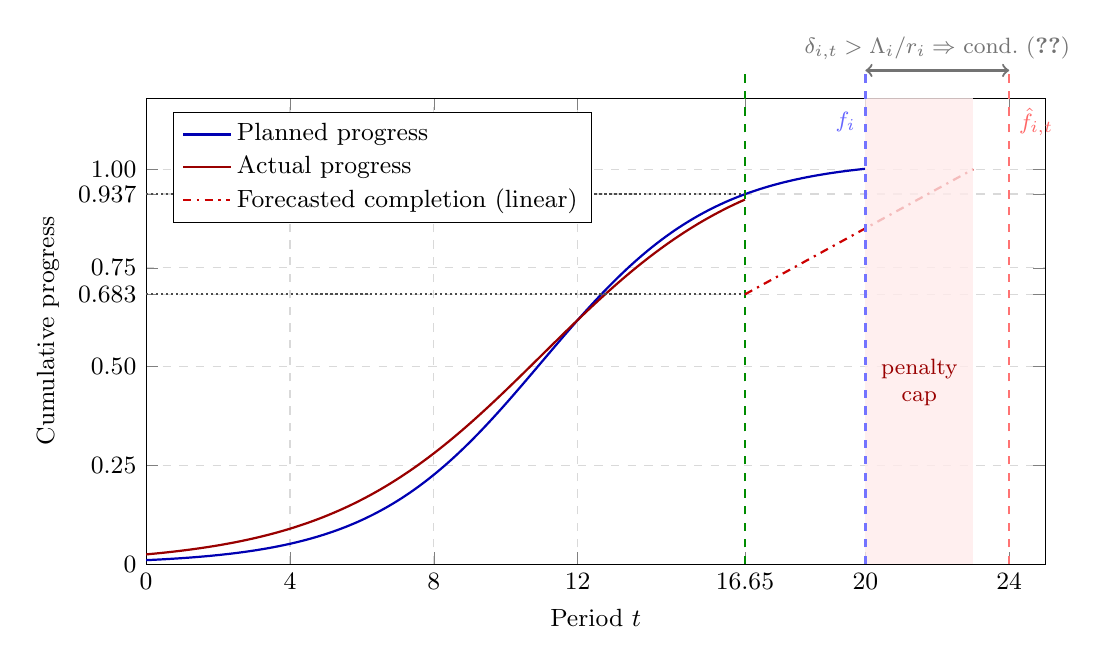
\begin{tikzpicture}
\begin{axis}[
    width=13cm, height=7.5cm,
    xlabel={Period $t$},
    ylabel={Cumulative progress},
    xmin=0, xmax=25,
    ymin=0, ymax=1.18,
    xtick={0,4,8,12,16.65,20,24},
    ytick={0,0.25,0.5,0.683,0.75,0.937,1.0},
    yticklabels={0,0.25,0.50,0.683,0.75,0.937,1.00},
    grid=major,
    grid style={dashed,gray!30},
    legend pos=north west,
    legend style={font=\small, cells={anchor=west}},
    tick label style={font=\small},
    label style={font=\small},
    clip=false,
  ]
  % ⚠️ this needs calibration. the actual curve must be expected to cross the threshold at an integer time

  \addplot[thick, blue!70!black, smooth, domain=0:20, samples=80]
    { (1/(1+exp(-0.42*(x-11)))) / 0.9767 };
  \addlegendentry{Planned progress}

  % \addplot[thick, red!60!black, smooth, domain=0:24, samples=80, dashed]
  %   { (0.88/(1+exp(-0.42*(x-15)))) / 0.860 };
  % \addlegendentry{Actual progress}
  
  \addplot[thick, red!60!black, smooth, domain=0:16.65, samples=80]
  { (1/(1+exp(-0.34*(x-11)))) / 0.945 };
  \addlegendentry{Actual progress}

  \draw[dashed, green!55!black, thick]
  (axis cs:16.65,0) -- (axis cs:16.65,1.25);

  \addplot[thick, red!80!black, dashdotted]
  coordinates {
    (16.65,0.683)
    (23,1)
  };
  \addlegendentry{Forecasted completion (linear)}

  \addplot[densely dotted, gray!60!black, thick]
  coordinates {(0,0.937)(16.65,0.937)};

  \addplot[densely dotted, gray!60!black, thick]
  coordinates {(0,0.683)(16.65,0.683)};
  
  \fill[red!8, opacity=0.8]
  (axis cs:20,0) rectangle (axis cs:23,1.18);
  \node[font=\footnotesize, red!60!black, align=center]
    at (axis cs:21.5,0.46)
    {penalty\\cap};

  \draw[dashed, blue!55, thick]
    (axis cs:20,0) -- (axis cs:20,1.25);
  \node[font=\footnotesize, blue!60, left]
    at (axis cs:20,1.12) {$f_i$};

  \draw[dashed, red!55, thick]
    (axis cs:24,0) -- (axis cs:24,1.25);
  \node[font=\footnotesize, red!60, right]
    at (axis cs:24,1.12) {$\hat{f}_{i,t}$};

  \draw[<->, thick, black!55]
    (axis cs:20,1.25) -- (axis cs:24,1.25)
    node[midway, above, font=\footnotesize]
      {$\delta_{i,t} > \Lambda_i/r_i \Rightarrow$ cond.~(\ref{eq:term_cond1})};

\end{axis}
\end{tikzpicture}
\caption{actual progress runs below, producing negative signed deviation $\delta_{i,t}$
  and values $\mathrm{SPI}_{i,t},\,\mathrm{CPI}_{i,t} < 1$. When the forecast
  finish gap $\hat{f}_{i,t}-f_i$ exceeds $\Lambda_i/r_i$ (shaded region),
  Termination Condition~(\ref{eq:term_cond1}) activates.}
\label{fig:scurve_evm}
\end{figure}

\FloatBarrier
\paragraph{Termination conditions and settlement.}
Termination is an endogenous environment mechanic. At each period $t$, the
environment evaluates two conditions for every active project $i$:
\begin{align}
  &\text{(i) Schedule tolerance exhausted:} \quad
    \hat{f}_{i,t} - f_i > \frac{\Lambda_i}{r_i},
  \label{eq:term_cond1} \\
  &\text{(ii) Cost performance unrecoverable:} \quad
    \mathrm{CPI}_{i,t} < \kappa_i,
  \label{eq:term_cond2}
\end{align}
where $\hat{f}_{i,t} = s_i + (D_i^{\mathrm{plan}} - (t - s_i)) /
\mathrm{SPI}_{i,t}$ is the linearly extrapolated forecast finish date and
$r_i$ is the per-period delay penalty rate. Condition~\eqref{eq:term_cond1}
signals that the forecast finish deviation has exceeded the maximum delay
the contract price can absorb before the penalty ceiling $\Lambda_i$ is
reached; Condition~\eqref{eq:term_cond2} signals that cost performance has
deteriorated below the project-specific recovery threshold $\kappa_i$.

When both conditions hold simultaneously, the environment decrements the
cure-period counter:
\begin{equation}
  \tau_{i,t}^{\mathrm{rem}} =
  \begin{cases}
    \tau_{i,t-1}^{\mathrm{rem}} - 1
      & \text{if \eqref{eq:term_cond1} and \eqref{eq:term_cond2} both hold,} \\
    \tau_i^{\mathrm{tol}}
      & \text{if either condition lapses.}
  \end{cases}
  \label{eq:counter}
\end{equation}
The counter initialises at $\tau_{i,s_i}^{\mathrm{rem}} = \tau_i^{\mathrm{tol}}$.
Termination executes at the period immediately following
$t_i^{\mathrm{term}} = \min\{t : \tau_{i,t}^{\mathrm{rem}} = 0\}$.
The counter is part of the observable state $S_t$; the agent cannot override
its dynamics but influences both conditions indirectly through allocation
decisions that drive $\mathrm{SPI}_{i,t}$ and $\mathrm{CPI}_{i,t}$.

\begin{figure}[htbp]
  \centering
  \resizebox{\textwidth}{!}{%
  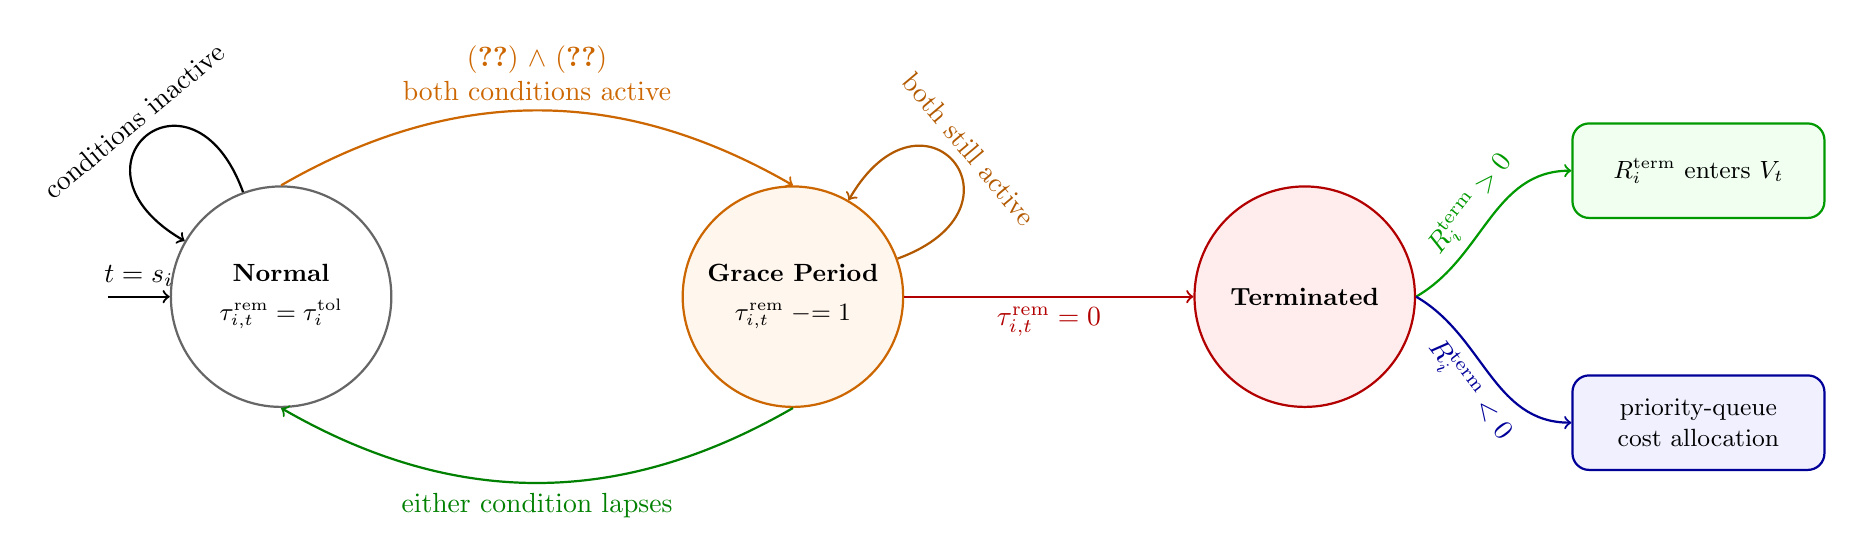
\begin{tikzpicture}[
      every node/.style={font=\small},
      state/.style={circle, draw=black!60, fill=white,
                    minimum size=2.8cm, align=center, thick},
      grace/.style={circle, draw=orange!80!black, fill=orange!7,
                    minimum size=2.8cm, align=center, thick},
      term/.style={circle, draw=red!70!black, fill=red!7,
                    minimum size=2.8cm, align=center, thick},
      posnode/.style={rectangle, rounded corners=6pt, draw=green!60!black,
                  fill=green!6, minimum width=3.2cm, minimum height=1.2cm,
                  align=center, thick},
      negnode/.style={rectangle, rounded corners=6pt, draw=blue!60!black,
                  fill=blue!6, minimum width=3.2cm, minimum height=1.2cm,
                  align=center, thick},
    ]
  
    \node[state] (normal) at (0,0)
      {\textbf{Normal}\\[3pt]
        $\tau_{i,t}^{\mathrm{rem}} = \tau_i^{\mathrm{tol}}$};
  
    \node[grace] (grace) at (6.5,0)
      {\textbf{Grace Period}\\[3pt]
        $\tau_{i,t}^{\mathrm{rem}} \mathrel{-}= 1$};
  
    \node[term] (term) at (13,0)
      {\textbf{Terminated}};
  
    \node[posnode] (posout) at (18,1.6)
      {$R_i^{\mathrm{term}}$ enters $V_t$};
  
    \node[negnode] (negout) at (18,-1.6)
      {priority-queue\\cost allocation};
  
    \draw[->, thick] (-2.2,0) -- (normal.west)
      node[midway, above, font=\normalsize] {$t = s_i$};
  
    \draw[->, thick, orange!80!black]
      (normal.north) to[out=30, in=150]
      node[above, font=\normalsize, align=center]
        {(\ref{eq:term_cond1}) $\wedge$ (\ref{eq:term_cond2})\\both conditions active}
      (grace.north);
  
    \draw[->, thick, green!50!black]
      (grace.south) to[out=210, in=330]
      node[below, font=\normalsize, align=center]
        {either condition lapses}
      (normal.south);
  
    \draw[->, thick, orange!70!black]
      (grace) to[out=20, in=60, looseness=5]
      node[above, font=\normalsize, sloped]
        {both still active}
      (grace);
  
    \draw[->, thick, red!70!black] (grace.east) -- (term.west)
      node[midway, below, font=\normalsize, align=center]
        {$\tau_{i,t}^{\mathrm{rem}} = 0$};
  
    \draw[->, thick, black]
      (normal) to[out=110, in=150, looseness=5]
      node[above, font=\normalsize, sloped] {conditions inactive}
      (normal);
  
    \draw[->, thick, green!60!black]
      (term.east) to[out=30, in=180]
      node[midway, above, font=\normalsize, sloped]
        {$R_i^{\mathrm{term}} > 0$}
      (posout.west);
  
    \draw[->, thick, blue!60!black]
      (term.east) to[out=-30, in=180]
      node[midway, below, font=\normalsize, sloped]
        {$R_i^{\mathrm{term}} < 0$}
      (negout.west);
  
  \end{tikzpicture}%
  }
  \caption{Finite-state representation of the termination mechanic for project $i$.}
  \label{fig:state_machine}
  \end{figure}

Upon termination at $t_i^{\mathrm{term}}$, the net settlement is:
\begin{equation}
  R_i^{\mathrm{term}}
    = P_{i,t_i^{\mathrm{term}}}^{\mathrm{actual}} \cdot CP_i (1-\rho_i)
      - \Bigl(A_i - \sum_{j \in \mathcal{M}_i^{\mathrm{cert}}(t_i^{\mathrm{term}})}
                \delta_i^{\mathrm{rec}} \cdot \phi_{i,j} \cdot CP_i
                \cdot \mathbf{1}\!\left\{\sum_{k \leq j} \phi_{i,k} \geq \psi_i\right\}
        \Bigr).
  \label{eq:term_settlement}
\end{equation}
Negative $R_i^{\mathrm{term}}$ (outstanding advance exceeds earned value)
constitutes a net obligation recovered from portfolio inflows, consistent with
FIDIC termination clauses \citep{FIDIC2017}.

\paragraph{Portfolio cash balance recursion.}
\begin{equation}
  B_{t+1} = B_t
    - \sum_{i \in \mathcal{P}_t^{\mathrm{active}}} x_{i,t}
    + V_t,
  \qquad B_t \geq 0 \quad \forall\,t \in \mathcal{T}.
  \label{eq:balance}
\end{equation}
The constraint $B_t \geq 0$ prohibits borrowing; the portfolio operates under
a fixed capital commitment \cite{kavadias2003resource}. The shared balance $B_t$
is the sole coupling across otherwise independent project dynamics, and its
linear scaling with $n$ characterizes the complexity that motivates the
intractability argument in Level~2.

% - - - - - - - - - - - - - - - - - - - - - - - - - - - - - -
\subsubsection{Shared Objective}
\label{subsubsec:objective}
% - - - - - - - - - - - - - - - - - - - - - - - - - - - - - -

The decision-maker maximizes discounted net cash flow over the horizon:
\begin{equation}
  \max_{\{x_{i,t}\}} \quad
  \mathbb{E}\!\left[
    \sum_{t=1}^{H} \gamma^{t-1}
    \!\left(
      V_t
      - \sum_{i \in \mathcal{P}_t^{\mathrm{active}}} x_{i,t}
      - \sum_{i \in \mathcal{P}_t^{\mathrm{active}}} c_{i,t}^{\mathrm{dev}}
    \right)
  \right],
  \label{eq:objective}
\end{equation}
subject to, for all $i \in \mathcal{P}$, $t \in \mathcal{T}$:
\begin{align}
  x_{i,t} &\geq 0,
  \label{eq:nonnegativity} \\
  \sum_{i \in \mathcal{P}_t^{\mathrm{active}}} x_{i,t} &\leq B_t,
  \label{eq:budget} \\
  x_{i,t} &= 0 \quad \text{if } \mathrm{status}_{i,t} \neq \texttt{active}.
  \label{eq:inactive}
\end{align}
There is no terminal sum. Completion incentives are embedded structurally:
$R_i^{\mathrm{ret}}$ and $R_{i,M_i}^{\mathrm{net}}$ enter $V_t$ at the
certification period; $R_i^{\mathrm{term}}$ (possibly negative) enters at
termination, creating a natural deterrent against allowing project performance
to deteriorate to the termination threshold.
Constraint~\eqref{eq:inactive} enforces that no budget is directed to
completed or terminated projects; the agent is free to allocate any
non-negative amount to active projects subject only to the shared
liquidity constraint~\eqref{eq:budget}.
The expectation $\mathbb{E}[\cdot]$ collapses to a deterministic
evaluation at Level~1 and is retained at Levels~2 and~3.

% ------------------------------------------------------------
\subsection{Level~1: Deterministic Full-Foresight MILP}
\label{subsec:level1}
% ------------------------------------------------------------

Setting $\eta_{i,t} = \bar{\eta}_{i,t}$ (known) renders $S_t$ a deterministic
function of $\mathbf{x}_t$, so $\mathcal{P}_t^{\mathrm{active}}$,
milestone certification times, and termination periods $t_i^{\mathrm{term}}$
are all computable ex ante. Introducing the certification binary
$u_{i,j,t} \in \{0,1\}$ ($=1$ iff milestone $j$ of project $i$ certified by
period $t$) and activity indicator $\mathrm{act}_{i,t} \in \{0,1\}$ (fixed
parameter), the stochastic objective~\eqref{eq:objective} collapses to the MILP:

\begin{subequations}
\label{eq:L1}
\begin{align}
  \max \quad
  & \sum_{t=1}^{H} \gamma^{t-1}\!\left(
      V_t^{\mathrm{det}}
      - \sum_{i \in \mathcal{P}} \mathrm{act}_{i,t}\, x_{i,t}
      - \sum_{i \in \mathcal{P}} \mathrm{act}_{i,t}\, c_{i,t}^{\mathrm{dev}}
    \right)
  \label{eq:L1_obj} \\[4pt]
%
  \text{s.t.} \quad
  B_{t+1} &= B_t
    - \sum_i \mathrm{act}_{i,t}\,x_{i,t} + V_t^{\mathrm{det}},
    \quad B_t \geq 0,
    && \forall\, t
  \label{eq:L1_balance} \\
%
  \sum_i \mathrm{act}_{i,t}\, x_{i,t} &\leq B_t,
    && \forall\, t
  \label{eq:L1_budget} \\
%
  P_{i,t}^{\mathrm{actual}}
    &= P_{i,t-1}^{\mathrm{actual}}
       + \bar{\eta}_{i,t}\,\tfrac{x_{i,t}}{\mathrm{BAC}_i},
    \quad P_{i,t}^{\mathrm{actual}} \leq 1,
    && \forall\, i,t
  \label{eq:L1_progress} \\
%
  P_{i,t}^{\mathrm{actual}}
    &\geq \theta_{i,j}\,u_{i,j,t} - \mathbf{M}(1 - u_{i,j,t}),
    && \forall\, i,j,t
  \label{eq:L1_cert_lb} \\
  P_{i,t}^{\mathrm{actual}}
    &\leq \theta_{i,j} + \mathbf{M}\,u_{i,j,t},
    \quad u_{i,j,t} \geq u_{i,j,t-1},
    \quad u_{i,j+1,t} \leq u_{i,j,t},
    && \forall\, i,j,t
  \label{eq:L1_cert_logic} \\
%
  V_t^{\mathrm{det}}
    &= \sum_{i,j} R_{i,j}^{\mathrm{net}}\,(u_{i,j,t} - u_{i,j,t-1})
       + \sum_i R_i^{\mathrm{ret}}\,(u_{i,M_i,t} - u_{i,M_i,t-1}) \notag \\
    &\quad + \sum_i A_i \cdot \mathbf{1}\{t{=}s_i\}
       + \sum_{i \in \mathcal{P}^{\mathrm{term}}} R_i^{\mathrm{term}}
         \cdot \mathbf{1}\{t{=}t_i^{\mathrm{term}}\},
    && \forall\, t
  \label{eq:L1_cashflow} \\
%
  \delta_{i,t}
    &= P_{i,t}^{\mathrm{actual}} - P_{i,t}^{\mathrm{plan}}
     = d_{i,t}^+ - d_{i,t}^-,
    \quad d_{i,t}^+, d_{i,t}^- \geq 0,
    && \forall\, i,t
  \label{eq:L1_dev_split} \\
  c_{i,t}^{\mathrm{dev}}
    &\geq \lambda_i(d_{i,t}^+ + d_{i,t}^-),
    \quad c_{i,t}^{\mathrm{dev}} \leq \Lambda_i \cdot CP_i,
    \quad c_{i,t}^{\mathrm{dev}} \geq 0,
    && \forall\, i,t
  \label{eq:L1_penalty_lin} \\
%
  x_{i,t}
    &= 0 \quad \text{if } \mathrm{act}_{i,t} = 0,
    && \forall\, i,t
  \label{eq:L1_inactive} \\
%
  x_{i,t} &\geq 0, \quad u_{i,j,t} \in \{0,1\},
    \quad u_{i,j,0} = P_{i,0}^{\mathrm{actual}} = 0.
    &&
  \label{eq:L1_domains}
\end{align}
\end{subequations}

The big-$M$ constant in \eqref{eq:L1_cert_lb}--\eqref{eq:L1_cert_logic}
is $\mathbf{M} = \max_{i,j}\theta_{i,j}$; tighter values may be derived
project-specifically. Constraints~\eqref{eq:L1_cert_lb}--\eqref{eq:L1_cert_logic}
implement the exact if-and-only-if certification logic with monotone, ordered
binary activation. Constraints~\eqref{eq:L1_dev_split}--\eqref{eq:L1_penalty_lin}
linearize the absolute-value and cap in \eqref{eq:penalty}: the maximizing
objective drives $c_{i,t}^{\mathrm{dev}}$ to the tighter of the two bounds,
recovering the exact symmetric penalty. The difference
$(u_{i,j,t} - u_{i,j,t-1})$ in \eqref{eq:L1_cashflow} equals one in the sole
period a milestone is first certified, linearizing the trigger without
additional binaries. Termination timing $t_i^{\mathrm{term}}$ and the
settlement $R_i^{\mathrm{term}}$ (\ref{eq:term_settlement}) are pre-computed
from $\bar{\eta}_{i,t}$ before solving: under deterministic efficiency, the
trajectories of $\mathrm{SPI}_{i,t}$, $\mathrm{CPI}_{i,t}$, and therefore
the counter $\tau_{i,t}^{\mathrm{rem}}$ are fully determined ex ante, so
both termination conditions \eqref{eq:term_cond1}--\eqref{eq:term_cond2}
and the counter dynamics \eqref{eq:counter} are parameter-verifiable at
Level~1. Termination periods and settlements enter the MILP as fixed
parameters rather than optimisation constraints, a simplification that
does not carry over to Levels~2--3 where termination timing is endogenous
to the stochastic trajectory.

\paragraph{Upper bound.}
Let $Z^*_{\mathrm{L1}}$ denote the Level~1 optimum. For any causal policy
$\pi$ feasible under uncertainty, $\sup_\pi \mathbb{E}[Z^\pi] \leq
Z^*_{\mathrm{L1}}$: every feasible causal allocation sequence is also feasible
in the Level~1 program solved on the realized trajectory, so the full-foresight
optimum dominates in expectation. The gap
$Z^*_{\mathrm{L1}} - Z^\pi$ quantifies the cost of uncertainty and anchors the
empirical comparison in Section~\ref{sec:experiments}.